\documentclass[a4paper]{article}

\usepackage[english]{babel}
\usepackage[utf8]{inputenc}
\usepackage{amsmath}
\usepackage{graphicx}
\usepackage[colorinlistoftodos]{todonotes}
\begin{document}
\begin{titlepage}
	\newcommand{\HRule}{\rule{\linewidth}{0.5mm}}
	\centering
	\textsc{\large VIETNAM GENERAL CONFEDERATION OF LABOUR \\
		\large \bfseries TON DUC THANG UNIVERSITY \\
		\large \bfseries Faculty of Information Technology}\\[1.0cm]
	
\includegraphics[width=5cm, height=2cm]{TDT} \\
	\vspace{5mm}
	\textsc{ \Large \bfseries SERVICE-ORIENTED ARCHITECTURE FINAL PROJECT}\\[1.5cm]
	{ \Large \bfseries INTERVIEW PROCESS MANAGER - SYSTEM REQUIREMENT}\\[1.0cm]
	\HRule \\[1.0cm]
	\vspace{20mm}
	\begin{minipage}{1.0\textwidth}
		\begin{flushright} \large
			\emph{Lecturer: \bfseries Phuc H. Duong, M.Sc} \\
			\emph{Author: \bfseries Tran Han Minh Khoa – 51503151
			} \\
			\emph{ \bfseries Vo Thanh Nhan – 51503128
			} \\
			\emph{ \bfseries Trinh Quoc Tan - 51603286} \\
		\end{flushright}
	\end{minipage}\\[2cm]
	
	{\large \today}\\[2cm]
\end{titlepage}



\begin{abstract}
Interview Process Management (IPM) is a program that helps automatically manage interview process in FPT Software from potential candidate management to the end of the process when candidates become official staff.
\end{abstract}

\section{Objective}
This System Requirement provides detail descriptions about all functional and non-functional requirements of the system. 

\section{Desctiption (Functoinal Requiment)}
- Receive and save request to database automatically. \\
- Able to manage the events had happened in the systems(logging). \\
- Able to update the interview results.
- Candidates can apply the interview from online form.
\subsection{Actor}
- Admin: The manager of the users informations.\\
- HR: Human Resource.\\
- Interviewer.

\subsection{Use Case}
- Login: Allow user to login to system.\\
- Manage Candidates: Allow user to manage candidates who are in interview.\\
- Manage Positions (Positions, Skills): Allow user to manage which position and skills candidates in the interview.  \\
- Manage Interviews Information: Allow user to manage details of the interview.\\
- Manage Users: Allow admin manage all users in the system.\\
- Logging: Save history of system.
\subsection{Relationship}
\begin{tabular}{|c|c|c|c|}
\hline 
Use Case - Actor & Admin & HR & Interviewer\\ 
\hline 
Login & x & x & x\\ 
\hline 
Manage Candidates & & x & x\\
\hline
Manage Positions & & x & \\
\hline
Manage Interviews Information & & x & \\
\hline
Manage Users & x & & \\
\hline
Logging & x & x & x\\
\hline
\end{tabular}

\section{Non-Functional Requiment}
- This system is built for internal use and only those who are granted accounts can be logged in and use the system with their roles.\\
- User accounts are only provided from the system admin.\\
- Each role has different function, and only the admin can authorize to account.\\
- Browsers: Microsoft Egde, Google Chrome, Mozilla Firefox.\\
- Operating system(OS): Windows 7, Windows 8.1, Windows 10.
\section{System Design}
\subsection{Use case Diagram}
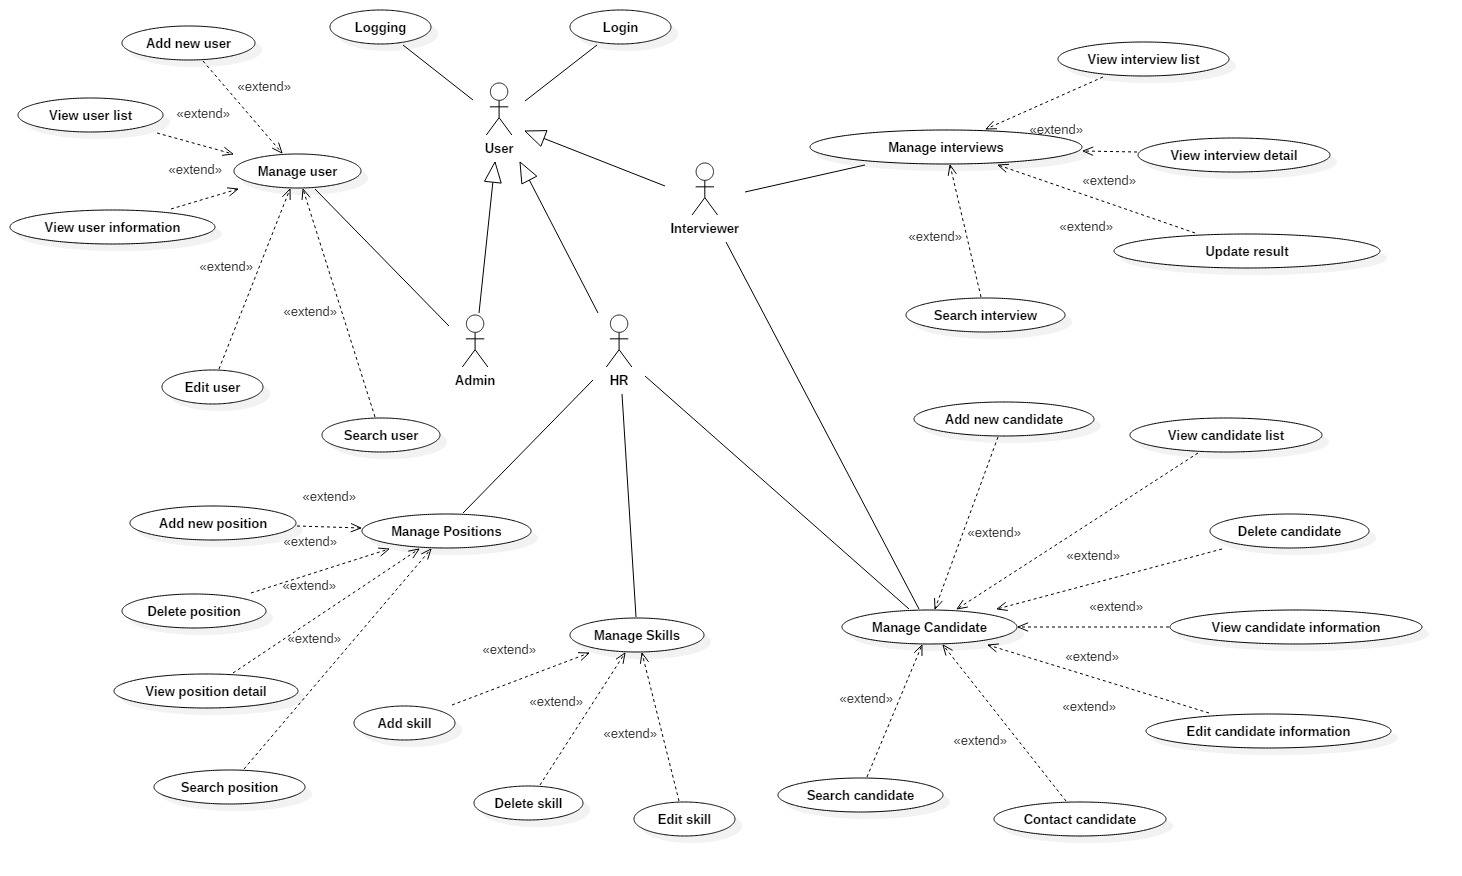
\includegraphics[width=15cm, height=10cm]{Diagram/UseCase} \\
\subsection{Use case Description}\

\subsubsection{Login}
\begin{tabular}{|l|p{5cm}||l|p{5cm}|}
	\hline 
	\multicolumn{2}{|p{5cm}|}{Usecase} & \multicolumn{2}{|p{5cm}|}{Login}\\ 
	\hline 
	\multicolumn{2}{|p{5cm}|}{Actor} & \multicolumn{2}{|p{5cm}|}{Admin, HR and Interviewer} \\ 
	\hline 
	\multicolumn{2}{|p{5cm}|}{Description} & \multicolumn{2}{|p{5cm}|}{login into the system}\\
	\hline
	\multicolumn{2}{|p{5cm}|}{Pre-condition} & \multicolumn{2}{|p{5cm}|}{Go to the url of system}\\
	\hline
	\multicolumn{2}{|p{5cm}|}{Post condition} & \multicolumn{2}{|p{5cm}|}{Login success} \\
	\hline
	\multicolumn{4}{|l|}{Main flow} \\
	\hline
	\multicolumn{2}{|p{5cm}|}{Actor} & \multicolumn{2}{|p{5cm}|}{System} \\
	\hline
	1 & Actor fill username and password & & \\
	\hline
	2 & Actor click login button & &  \\
	\hline
	& & 3 & The system check username and password with database \\
	\hline 
	& & 4 & The system send message "login success"  \\
	\hline
\end{tabular}

\subsubsection{Log out}
\begin{tabular}{|l|p{5cm}||l|p{5cm}|}
	\hline 
	\multicolumn{2}{|p{5cm}|}{Usecase} & \multicolumn{2}{|p{5cm}|}{Log out}\\ 
	\hline 
	\multicolumn{2}{|p{5cm}|}{Actor} & \multicolumn{2}{|p{5cm}|}{Admin, HR and Interviewer} \\ 
	\hline 
	\multicolumn{2}{|p{5cm}|}{Description} & \multicolumn{2}{|p{5cm}|}{log out of the system}\\
	\hline
	\multicolumn{2}{|p{5cm}|}{Pre-condition} & \multicolumn{2}{|p{5cm}|}{Login succeed}\\
	\hline
	\multicolumn{2}{|p{5cm}|}{Post condition} & \multicolumn{2}{|p{5cm}|}{Log out success} \\
	\hline
	\multicolumn{4}{|l|}{Main flow} \\
	\hline
	\multicolumn{2}{|p{5cm}|}{Actor} & \multicolumn{2}{|p{5cm}|}{System} \\
	\hline
	1 & Actor click login button & &  \\
	\hline
	& & 2 & The system logout the actor out of system  \\
	\hline 
	& & 3 & The system send message "logout success"  \\
	\hline
\end{tabular}

\subsubsection{Logging}
\begin{tabular}{|l|p{5cm}||l|p{5cm}|}
	\hline 
	\multicolumn{2}{|p{5cm}|}{Usecase} & \multicolumn{2}{|p{5cm}|}{Logging}\\ 
	\hline 
	\multicolumn{2}{|p{5cm}|}{Actor} & \multicolumn{2}{|p{5cm}|}{Admin, HR and Interviewer} \\ 
	\hline 
	\multicolumn{2}{|p{5cm}|}{Description} & \multicolumn{2}{|p{5cm}|}{Records activity log}\\
	\hline
	\multicolumn{2}{|p{5cm}|}{Pre-condition} & \multicolumn{2}{|p{5cm}|}{Login succeed}\\
	\hline
	\multicolumn{2}{|p{5cm}|}{Post condition} & \multicolumn{2}{|p{5cm}|}{Records activity log of actor} \\
	\hline
	\multicolumn{4}{|l|}{Main flow} \\
	\hline
	\multicolumn{2}{|p{5cm}|}{Actor} & \multicolumn{2}{|p{5cm}|}{System} \\
	\hline
	1 & Actor login into the system & & \\
	\hline
	& & 2 & The system record activities log of actor \\
	\hline
\end{tabular}

\subsubsection{Manage Users}
\begin{tabular}{|l|p{5cm}||l|p{5cm}|}
	\hline 
	\multicolumn{2}{|p{5cm}|}{Usecase} & \multicolumn{2}{|p{5cm}|}{Manage Users}\\ 
	\hline 
	\multicolumn{2}{|p{5cm}|}{Actor} & \multicolumn{2}{|p{5cm}|}{Admin} \\ 
	\hline 
	\multicolumn{2}{|p{5cm}|}{Description} & \multicolumn{2}{|p{5cm}|}{Views users list, add, delete, or update user in list}\\
	\hline
	\multicolumn{2}{|p{5cm}|}{Pre-condition} & \multicolumn{2}{|p{5cm}|}{Login succeed}\\
	\hline
	\multicolumn{2}{|p{5cm}|}{Post condition} & \multicolumn{2}{|p{5cm}|}{Displays the users list} \\
	\hline
	\multicolumn{4}{|l|}{Main flow} \\
	\hline
	\multicolumn{2}{|p{5cm}|}{Actor} & \multicolumn{2}{|p{5cm}|}{System} \\
	\hline
	1 & Admin choose Manage Users & & \\
	\hline
	& & 2 & The system queries the database \\
	\hline 
	& & 3 & the system shows users list  \\
	\hline		
\end{tabular}

\subsubsection{Manage Candidates}
\begin{tabular}{|l|p{5cm}||l|p{5cm}|}
	\hline 
	\multicolumn{2}{|p{5cm}|}{Usecase} & \multicolumn{2}{|p{5cm}|}{Manage Candidates}\\ 
	\hline 
	\multicolumn{2}{|p{5cm}|}{Actor} & \multicolumn{2}{|p{5cm}|}{HR and Interviewer} \\ 
	\hline 
	\multicolumn{2}{|p{5cm}|}{Description} & \multicolumn{2}{|p{5cm}|}{views candidates list}\\
	\hline
	\multicolumn{2}{|p{5cm}|}{Pre-condition} & \multicolumn{2}{|p{5cm}|}{Login succeed}\\
	\hline
	\multicolumn{2}{|p{5cm}|}{Post condition} & \multicolumn{2}{|p{5cm}|}{Displays the candidates list} \\
	\hline
	\multicolumn{4}{|l|}{Main flow} \\
	\hline
	\multicolumn{2}{|p{5cm}|}{Actor} & \multicolumn{2}{|p{5cm}|}{System} \\
	\hline
	1 & Actor choose Manage Candidates & & \\
	\hline
	& & 2 & The system queries to the Database \\
	\hline 
	& & 3 & The system shows the candidates list  \\
	\hline
\end{tabular}

\subsubsection{Manage Skills}
\begin{tabular}{|l|p{5cm}||l|p{5cm}|}
	\hline 
	\multicolumn{2}{|p{5cm}|}{Usecase} & \multicolumn{2}{|p{5cm}|}{Manage Skills}\\ 
	\hline 
	\multicolumn{2}{|p{5cm}|}{Actor} & \multicolumn{2}{|p{5cm}|}{HR} \\ 
	\hline 
	\multicolumn{2}{|p{5cm}|}{Description} & \multicolumn{2}{|p{5cm}|}{View skills list}\\
	\hline
	\multicolumn{2}{|p{5cm}|}{Pre-condition} & \multicolumn{2}{|p{5cm}|}{Login succeed}\\
	\hline
	\multicolumn{2}{|p{5cm}|}{Post condition} & \multicolumn{2}{|p{5cm}|}{Displays the skills list} \\
	\hline
	\multicolumn{4}{|l|}{Main flow} \\
	\hline
	\multicolumn{2}{|p{5cm}|}{Actor} & \multicolumn{2}{|p{5cm}|}{System} \\
	\hline
	1 & HR choose Manage Skills & & \\
	\hline
	& & 2 & The system queries to the database \\
	\hline 
	& & 3 & The system shows skills list  \\
	\hline
\end{tabular}

\subsubsection{Manage Positions}
\begin{tabular}{|l|p{5cm}||l|p{5cm}|}
	\hline 
	\multicolumn{2}{|p{5cm}|}{Usecase} & \multicolumn{2}{|p{5cm}|}{Manage Positions}\\ 
	\hline 
	\multicolumn{2}{|p{5cm}|}{Actor} & \multicolumn{2}{|p{5cm}|}{HR} \\ 
	\hline 
	\multicolumn{2}{|p{5cm}|}{Description} & \multicolumn{2}{|p{5cm}|}{View Positions list}\\
	\hline
	\multicolumn{2}{|p{5cm}|}{Pre-condition} & \multicolumn{2}{|p{5cm}|}{Login succeed}\\
	\hline
	\multicolumn{2}{|p{5cm}|}{Post condition} & \multicolumn{2}{|p{5cm}|}{Displays the positions list} \\
	\hline
	\multicolumn{4}{|l|}{Main flow} \\
	\hline
	\multicolumn{2}{|p{5cm}|}{Actor} & \multicolumn{2}{|p{5cm}|}{System} \\
	\hline
	1 & HR choose Manage Positions & & \\
	\hline
	& & 2 & The system queries to the database \\
	\hline 
	& & 3 & The system shows postions list  \\
	\hline
\end{tabular}

\subsubsection{Manage Interviews}
\begin{tabular}{|l|p{5cm}||l|p{5cm}|}
	\hline 
	\multicolumn{2}{|p{5cm}|}{Usecase} & \multicolumn{2}{|p{5cm}|}{Manage Interviews}\\ 
	\hline 
	\multicolumn{2}{|p{5cm}|}{Actor} & \multicolumn{2}{|p{5cm}|}{Interviewer} \\ 
	\hline 
	\multicolumn{2}{|p{5cm}|}{Description} & \multicolumn{2}{|p{5cm}|}{View interviews list}\\
	\hline
	\multicolumn{2}{|p{5cm}|}{Pre-condition} & \multicolumn{2}{|p{5cm}|}{Login succeed}\\
	\hline
	\multicolumn{2}{|p{5cm}|}{Post condition} & \multicolumn{2}{|p{5cm}|}{Displays the interviews list} \\
	\hline
	\multicolumn{4}{|l|}{Main flow} \\
	\hline
	\multicolumn{2}{|p{5cm}|}{Actor} & \multicolumn{2}{|p{5cm}|}{System} \\
	\hline
	1 & Interviewer choose Manage Interviews & & \\
	\hline
	& & 2 & The system queries to the database \\
	\hline 
	& & 3 & The system shows interviews list  \\
	\hline
\end{tabular}
\subsubsection{Add New User}
\begin{tabular}{|l|p{5cm}||l|p{5cm}|}
	\hline 
	\multicolumn{2}{|p{5cm}|}{Usecase} & \multicolumn{2}{|p{5cm}|}{Add New User}\\ 
	\hline 
	\multicolumn{2}{|p{5cm}|}{Actor} & \multicolumn{2}{|p{5cm}|}{Admin} \\ 
	\hline 
	\multicolumn{2}{|p{5cm}|}{Description} & \multicolumn{2}{|p{5cm}|}{Add new user into users list}\\
	\hline
	\multicolumn{2}{|p{5cm}|}{Pre-condition} & \multicolumn{2}{|p{5cm}|}{Login succeed, is on page "Manage Users"}\\
	\hline
	\multicolumn{2}{|p{5cm}|}{Post condition} & \multicolumn{2}{|p{5cm}|}{Add new user successfully} \\
	\hline
	\multicolumn{4}{|l|}{Main flow} \\
	\hline
	\multicolumn{2}{|p{5cm}|}{Actor} & \multicolumn{2}{|p{5cm}|}{System} \\
	\hline
	1 & Admin choose Add New User & & \\
	\hline
	& & 2 & Load page "Add New User" \\
	\hline 
	3 & Enter required information & & \\	
	\hline
	& & 4 &System validate entered information \\	
	\hline 
	5 & Edit information if system check it's not correct. & & \\	
	\hline
	& & 6 &Save information of new user into database.\\
	& &  &Notification add successfully.\\
	& & &Navigate to the page Manage User. \\	
	\hline 	
\end{tabular}
\subsubsection{Delete User}
\begin{tabular}{|l|p{5cm}||l|p{5cm}|}
	\hline 
	\multicolumn{2}{|p{5cm}|}{Usecase} & \multicolumn{2}{|p{5cm}|}{Delete User}\\ 
	\hline 
	\multicolumn{2}{|p{5cm}|}{Actor} & \multicolumn{2}{|p{5cm}|}{Admin} \\ 
	\hline 
	\multicolumn{2}{|p{5cm}|}{Description} & \multicolumn{2}{|p{5cm}|}{Remove user from users list}\\
	\hline
	\multicolumn{2}{|p{5cm}|}{Pre-condition} & \multicolumn{2}{|p{5cm}|}{Login succeed, is on page "Manage Users", is selecting user}\\
	\hline
	\multicolumn{2}{|p{5cm}|}{Post condition} & \multicolumn{2}{|p{5cm}|}{Delete user successfully} \\
	\hline
	\multicolumn{4}{|l|}{Main flow} \\
	\hline
	\multicolumn{2}{|p{5cm}|}{Actor} & \multicolumn{2}{|p{5cm}|}{System} \\
	\hline
	1 & Admin choose button Delete & & \\
	\hline
 	& & 2 & Delete user from database \\
	& &  &Notification delete successfully.\\
	& & &Navigate to the page Manage User. \\	
	\hline 	
\end{tabular}
\subsubsection{Update User Information}
\begin{tabular}{|l|p{5cm}||l|p{5cm}|}
	\hline 
	\multicolumn{2}{|p{5cm}|}{Usecase} & \multicolumn{2}{|p{5cm}|}{Update User Information}\\ 
	\hline 
	\multicolumn{2}{|p{5cm}|}{Actor} & \multicolumn{2}{|p{5cm}|}{Admin} \\ 
	\hline 
	\multicolumn{2}{|p{5cm}|}{Description} & \multicolumn{2}{|p{5cm}|}{Update all information of choosing user}\\
	\hline
	\multicolumn{2}{|p{5cm}|}{Pre-condition} & \multicolumn{2}{|p{5cm}|}{Login succeed, is on page "Manage Users"}\\
	\hline
	\multicolumn{2}{|p{5cm}|}{Post condition} & \multicolumn{2}{|p{5cm}|}{Load user information page to review.} \\
	\hline
	\multicolumn{4}{|l|}{Main flow} \\
	\hline
	\multicolumn{2}{|p{5cm}|}{Actor} & \multicolumn{2}{|p{5cm}|}{System} \\
	\hline
	1 & Admin choose button Update & & \\
	\hline
	& & 2 & Display current user information detail page \\
	\hline
	3 & Update user information & & \\
	\hline
	4 & Click button Update & & \\
	\hline	
	& & 5 &Update user information in database. \\	
	\hline 			
\end{tabular}
\subsubsection{Add New Candidate}
\begin{tabular}{|l|p{5cm}||l|p{5cm}|}
	\hline 
	\multicolumn{2}{|p{5cm}|}{Usecase} & \multicolumn{2}{|p{5cm}|}{Add New Candidate}\\ 
	\hline 
	\multicolumn{2}{|p{5cm}|}{Actor} & \multicolumn{2}{|p{5cm}|}{HR, Interviewer} \\ 
	\hline 
	\multicolumn{2}{|p{5cm}|}{Description} & \multicolumn{2}{|p{5cm}|}{Add new candidate into candiate list}\\
	\hline
	\multicolumn{2}{|p{5cm}|}{Pre-condition} & \multicolumn{2}{|p{5cm}|}{Login succeed, is on page "Manage Candidates"}\\
	\hline
	\multicolumn{2}{|p{5cm}|}{Post condition} & \multicolumn{2}{|p{5cm}|}{Add new candidate successfully} \\
	\hline
	\multicolumn{4}{|l|}{Main flow} \\
	\hline
	\multicolumn{2}{|p{5cm}|}{Actor} & \multicolumn{2}{|p{5cm}|}{System} \\
	\hline
	1 & Admin choose Add New Candidate & & \\
	\hline
	& & 2 & Load page "Add New Candidate" \\
	\hline 
	3 & Enter required information & & \\	
	\hline
	& & 4 &System validate entered information \\	
	\hline 
	5 & Edit information if system check it's not correct. & & \\	
	\hline
	& & 6 &Save information of new candidate into database.\\
	& &  &Notification add successfully.\\
	& & &Navigate to the page Manage Candidate. \\	
	\hline 	
\end{tabular}
\subsubsection{Delete Candidate}
\begin{center}
\begin{tabular}{|l|p{5cm}||l|p{5cm}|}
	\hline 
	\multicolumn{2}{|p{5cm}|}{Usecase} & \multicolumn{2}{|p{5cm}|}{Delete Candidate}\\ 
	\hline 
	\multicolumn{2}{|p{5cm}|}{Actor} & \multicolumn{2}{|p{5cm}|}{HR, Interviewer} \\ 
	\hline 
	\multicolumn{2}{|p{5cm}|}{Description} & \multicolumn{2}{|p{5cm}|}{Remove candidate from users list}\\
	\hline
	\multicolumn{2}{|p{5cm}|}{Pre-condition} & \multicolumn{2}{|p{5cm}|}{Login succeed, on page "Manage Candidates"}\\
	\hline
	\multicolumn{2}{|p{5cm}|}{Post condition} & \multicolumn{2}{|p{5cm}|}{Delete candidate successfully} \\
	\hline
	\multicolumn{4}{|l|}{Main flow} \\
	\hline
	\multicolumn{2}{|p{5cm}|}{Actor} & \multicolumn{2}{|p{5cm}|}{System} \\
	\hline
	1 & Admin choose button Delete & & \\
	\hline
	& & 2 & Delete candidate from database \\
	& &  &Notification delete successfully.\\
	& & &Navigate to the page Manage Candidate. \\	
	\hline 	
\end{tabular}
\end{center}
\subsubsection{Update Candidate Information}
\begin{tabular}{|l|p{5cm}||l|p{5cm}|}
	\hline 
	\multicolumn{2}{|p{5cm}|}{Usecase} & \multicolumn{2}{|p{5cm}|}{Update Candidate Information}\\ 
	\hline 
	\multicolumn{2}{|p{5cm}|}{Actor} & \multicolumn{2}{|p{5cm}|}{HR, Interviewer} \\ 
	\hline 
	\multicolumn{2}{|p{5cm}|}{Description} & \multicolumn{2}{|p{5cm}|}{Update all information of choosing candidate}\\
	\hline
	\multicolumn{2}{|p{5cm}|}{Pre-condition} & \multicolumn{2}{|p{5cm}|}{Login succeed, is on page "Manage Candidates"}\\
	\hline
	\multicolumn{2}{|p{5cm}|}{Post condition} & \multicolumn{2}{|p{5cm}|}{Load candidate information page to review.} \\
	\hline
	\multicolumn{4}{|l|}{Main flow} \\
	\hline
	\multicolumn{2}{|p{5cm}|}{Actor} & \multicolumn{2}{|p{5cm}|}{System} \\
	\hline
	1 & Admin choose button Update & & \\
	\hline
	& & 2 & Display current candidate information detail page \\
	\hline
	3 & Update candidate information & & \\
	\hline
	4 & Click button Update & & \\
	\hline	
	& & 5 &Update candidate information in database. \\	
	\hline 			
\end{tabular}
\subsubsection{Contact Candidate}
\begin{tabular}{|l|p{5cm}||l|p{5cm}|}
	\hline 
	\multicolumn{2}{|p{5cm}|}{Usecase} & \multicolumn{2}{|p{5cm}|}{Contact Candidate}\\ 
	\hline 
	\multicolumn{2}{|p{5cm}|}{Actor} & \multicolumn{2}{|p{5cm}|}{HR and Interviewer} \\ 
	\hline 
	\multicolumn{2}{|p{5cm}|}{Description} & \multicolumn{2}{|p{5cm}|}{Make an appointment for an interview}\\
	\hline
	\multicolumn{2}{|p{5cm}|}{Pre-condition} & \multicolumn{2}{|p{5cm}|}{Login succeed, on page "Manage Candidates"}\\
	\hline
	\multicolumn{2}{|p{5cm}|}{Post condition} & \multicolumn{2}{|p{5cm}|}{Make an appointment for an interview success} \\
	\hline
	\multicolumn{4}{|l|}{Main flow} \\
	\hline
	\multicolumn{2}{|p{5cm}|}{Actor} & \multicolumn{2}{|p{5cm}|}{System} \\
	\hline
	1 & clicks the button "Contact" & & \\
	\hline
	& & 2 & displays contact form" \\
	\hline 
	3 & fills contact information and click "send" &  &  \\
	\hline
	& & 4 & sends to candidate an email about interview datetime \\
	\hline
\end{tabular}
\subsubsection{Search Candidate}
\begin{tabular}{|l|p{5cm}||l|p{5cm}|}
	\hline 
	\multicolumn{2}{|p{5cm}|}{Usecase} & \multicolumn{2}{|p{5cm}|}{Search Candidate}\\ 
	\hline 
	\multicolumn{2}{|p{5cm}|}{Actor} & \multicolumn{2}{|p{5cm}|}{HR and Interviewer} \\ 
	\hline 
	\multicolumn{2}{|p{5cm}|}{Description} & \multicolumn{2}{|p{5cm}|}{Search candidate or candidates}\\
	\hline
	\multicolumn{2}{|p{5cm}|}{Pre-condition} & \multicolumn{2}{|p{5cm}|}{Login succeed, on page "Manage Candidates"}\\
	\hline
	\multicolumn{2}{|p{5cm}|}{Post condition} & \multicolumn{2}{|p{5cm}|}{find candidate allow keyword} \\
	\hline
	\multicolumn{4}{|l|}{Main flow} \\
	\hline
	\multicolumn{2}{|p{5cm}|}{Actor} & \multicolumn{2}{|p{5cm}|}{System} \\
	\hline
	1 & fill keyword into input box & & \\
	\hline
	& & 2 & find all candidates have keyword  \\
	\hline 
\end{tabular}
\subsubsection{Add New Position}
\begin{tabular}{|l|p{5cm}||l|p{5cm}|}
	\hline 
	\multicolumn{2}{|p{5cm}|}{Usecase} & \multicolumn{2}{|p{5cm}|}{Add New Position}\\ 
	\hline 
	\multicolumn{2}{|p{5cm}|}{Actor} & \multicolumn{2}{|p{5cm}|}{HR} \\ 
	\hline 
	\multicolumn{2}{|p{5cm}|}{Description} & \multicolumn{2}{|p{5cm}|}{Add new position into position list}\\
	\hline
	\multicolumn{2}{|p{5cm}|}{Pre-condition} & \multicolumn{2}{|p{5cm}|}{Login succeed, is on page "Manage Positions"}\\
	\hline
	\multicolumn{2}{|p{5cm}|}{Post condition} & \multicolumn{2}{|p{5cm}|}{Add new position successfully} \\
	\hline
	\multicolumn{4}{|l|}{Main flow} \\
	\hline
	\multicolumn{2}{|p{5cm}|}{Actor} & \multicolumn{2}{|p{5cm}|}{System} \\
	\hline
	1 & Admin choose Add New Positions & & \\
	\hline
	& & 2 & Load page "Add New Position" \\
	\hline 
	3 & Enter required information & & \\	
	\hline
	& & 4 &System validate entered information \\	
	\hline 
	5 & Edit information if system check it's not correct. & & \\	
	\hline
	& & 6 &Save information of new position into database.\\
	& &  &Notification add successfully.\\
	& & &Navigate to the page Manage Positions. \\	
	\hline 	
\end{tabular}
\subsubsection{Delete Position}
\begin{tabular}{|l|p{5cm}||l|p{5cm}|}
	\hline 
	\multicolumn{2}{|p{5cm}|}{Usecase} & \multicolumn{2}{|p{5cm}|}{Delete Position}\\ 
	\hline 
	\multicolumn{2}{|p{5cm}|}{Actor} & \multicolumn{2}{|p{5cm}|}{HR} \\ 
	\hline 
	\multicolumn{2}{|p{5cm}|}{Description} & \multicolumn{2}{|p{5cm}|}{Remove position from users list}\\
	\hline
	\multicolumn{2}{|p{5cm}|}{Pre-condition} & \multicolumn{2}{|p{5cm}|}{Login succeed, is on page "Manage Positions", is selecting position}\\
	\hline
	\multicolumn{2}{|p{5cm}|}{Post condition} & \multicolumn{2}{|p{5cm}|}{Delete position successfully} \\
	\hline
	\multicolumn{4}{|l|}{Main flow} \\
	\hline
	\multicolumn{2}{|p{5cm}|}{Actor} & \multicolumn{2}{|p{5cm}|}{System} \\
	\hline
	1 & Admin choose button Delete & & \\
	\hline
	& & 2 & Delete position from database \\
	& &  &Notification delete successfully.\\
	& & &Navigate to the page Manage Positions. \\	
	\hline 	
\end{tabular}
\subsubsection{Update Position Information}
\begin{tabular}{|l|p{5cm}||l|p{5cm}|}
	\hline 
	\multicolumn{2}{|p{5cm}|}{Usecase} & \multicolumn{2}{|p{5cm}|}{Update Position Information}\\ 
	\hline 
	\multicolumn{2}{|p{5cm}|}{Actor} & \multicolumn{2}{|p{5cm}|}{HR} \\ 
	\hline 
	\multicolumn{2}{|p{5cm}|}{Description} & \multicolumn{2}{|p{5cm}|}{Update all information of choosing position}\\
	\hline
	\multicolumn{2}{|p{5cm}|}{Pre-condition} & \multicolumn{2}{|p{5cm}|}{Login succeed, is on page "Manage Positions"}\\
	\hline
	\multicolumn{2}{|p{5cm}|}{Post condition} & \multicolumn{2}{|p{5cm}|}{Load position information page to review.} \\
	\hline
	\multicolumn{4}{|l|}{Main flow} \\
	\hline
	\multicolumn{2}{|p{5cm}|}{Actor} & \multicolumn{2}{|p{5cm}|}{System} \\
	\hline
	1 & Admin choose button Update & & \\
	\hline
	& & 2 & Display current position information detail page \\
	\hline
	3 & Update candidate information & & \\
	\hline
	4 & Click button Update & & \\
	\hline	
	& & 5 &Update position information in database. \\	
	\hline 			
\end{tabular}
\subsubsection{Search Interview}
\begin{tabular}{|l|p{5cm}||l|p{5cm}|}
	\hline 
	\multicolumn{2}{|p{5cm}|}{Usecase} & \multicolumn{2}{|p{5cm}|}{Search Interview}\\ 
	\hline 
	\multicolumn{2}{|p{5cm}|}{Actor} & \multicolumn{2}{|p{5cm}|}{Interviewer} \\ 
	\hline 
	\multicolumn{2}{|p{5cm}|}{Description} & \multicolumn{2}{|p{5cm}|}{Search interview}\\
	\hline
	\multicolumn{2}{|p{5cm}|}{Pre-condition} & \multicolumn{2}{|p{5cm}|}{Login succeed, on page "Manage Interviews"}\\
	\hline
	\multicolumn{2}{|p{5cm}|}{Post condition} & \multicolumn{2}{|p{5cm}|}{find out the interview with keyword} \\
	\hline
	\multicolumn{4}{|l|}{Main flow} \\
	\hline
	\multicolumn{2}{|p{5cm}|}{Actor} & \multicolumn{2}{|p{5cm}|}{System} \\
	\hline
	1 & fills keyword into searching box & & \\
	\hline
	& & 2 & finds the interviews have keyword \\
	\hline 
\end{tabular}



\subsection{Class Diagram}
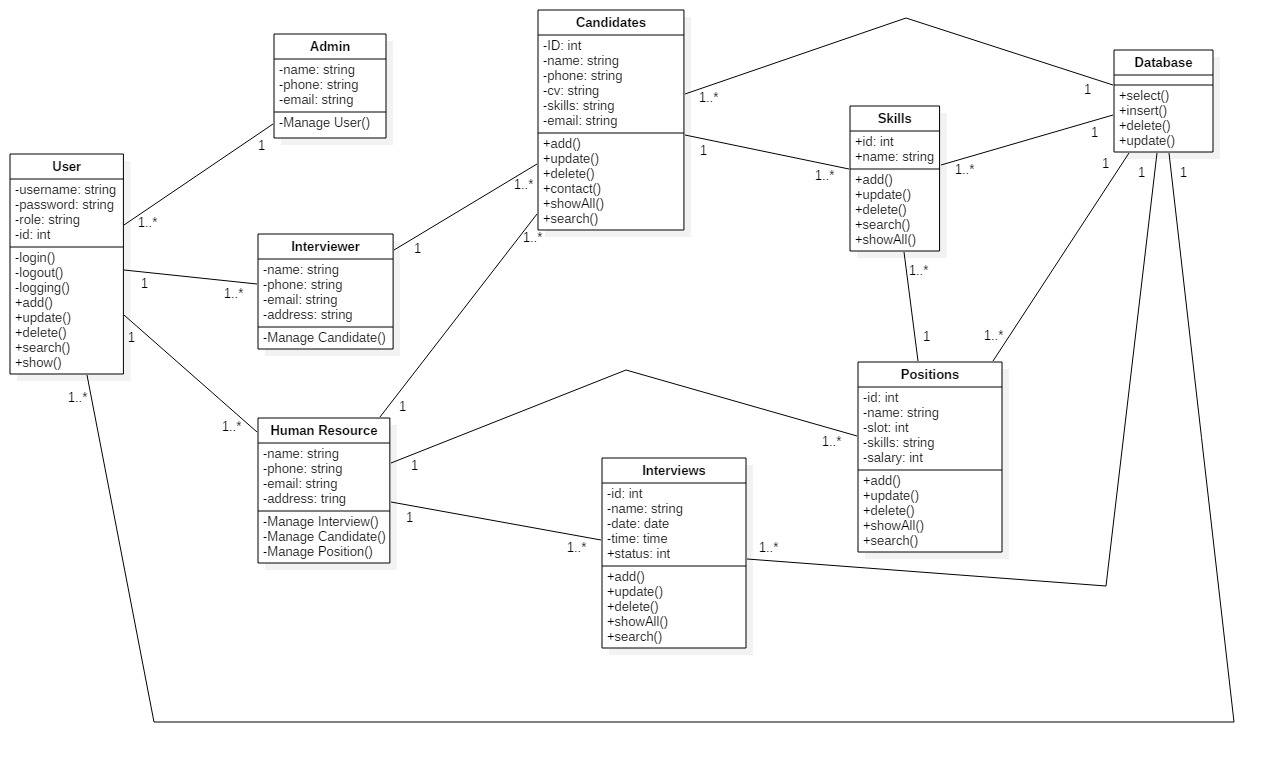
\includegraphics[width=15cm, height=10cm]{Diagram/Class} \\
\subsection{Sequence Diagram}
\subsubsection{Manage Users}
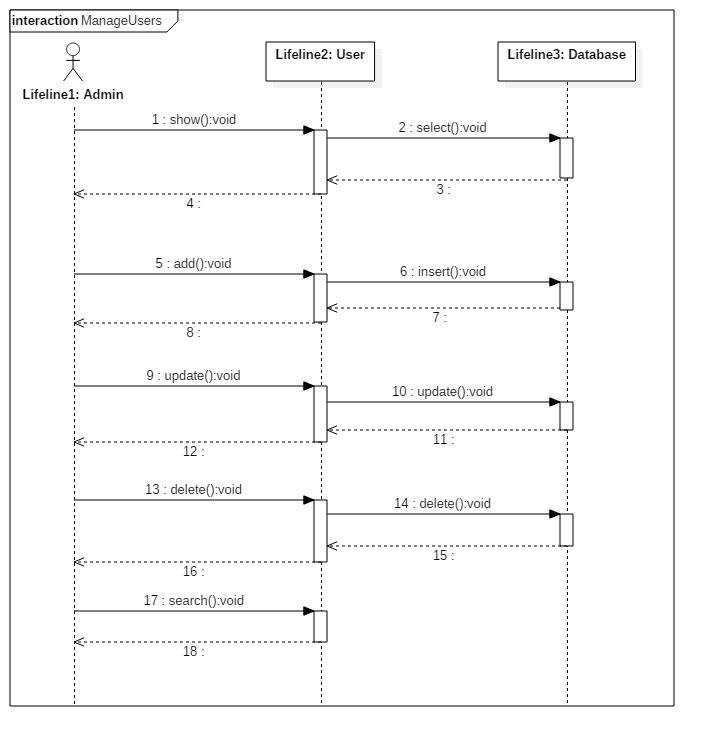
\includegraphics[width=15cm, height=10cm]{Diagram/ManageUser} \\
\subsubsection{Manage Candidates}
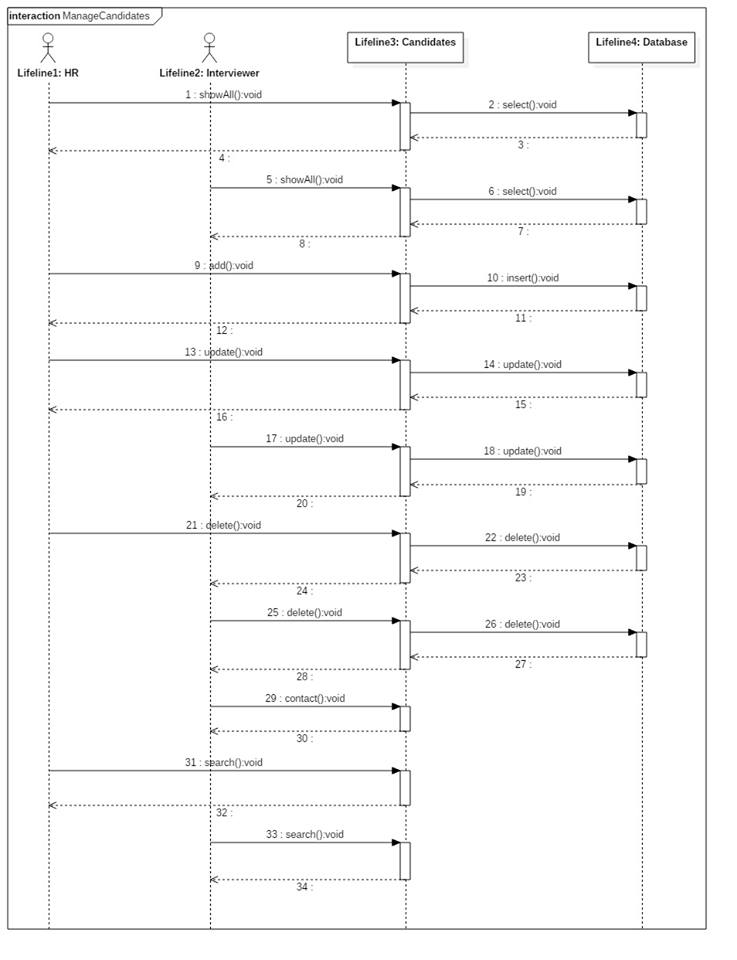
\includegraphics[width=15cm, height=10cm]{Diagram/ManageCandidate} \\
\subsubsection{Manage Interviews}
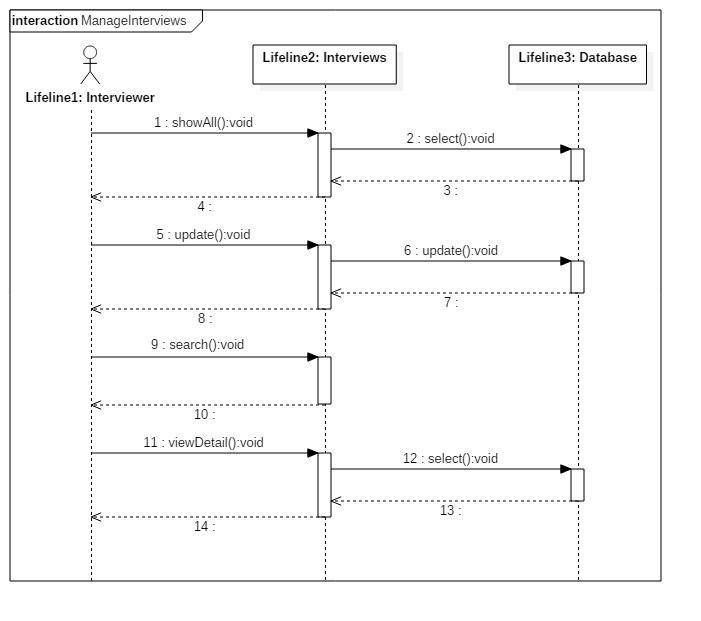
\includegraphics[width=15cm, height=10cm]{Diagram/ManageInterview} \\
\subsubsection{Manage Positions}
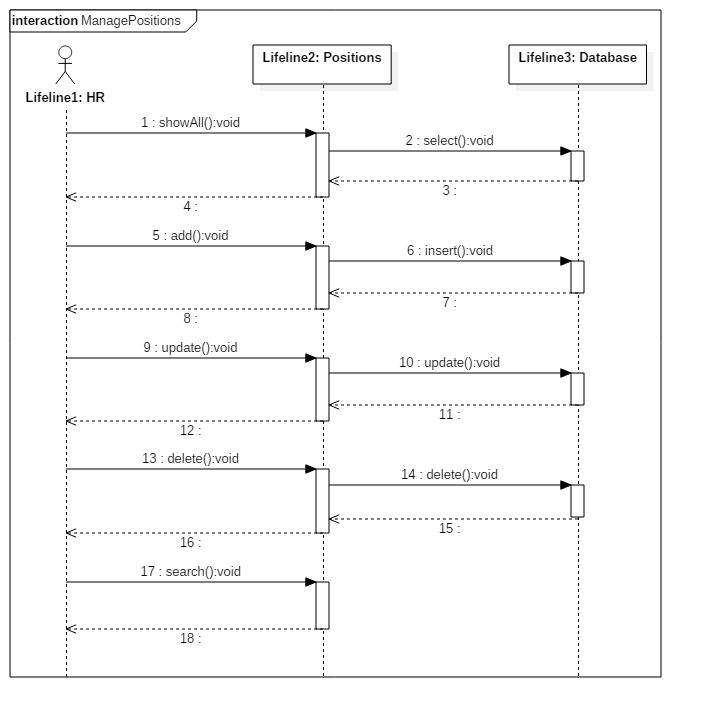
\includegraphics[width=15cm, height=10cm]{Diagram/ManagePos} \\
\subsubsection{Manage Skills}
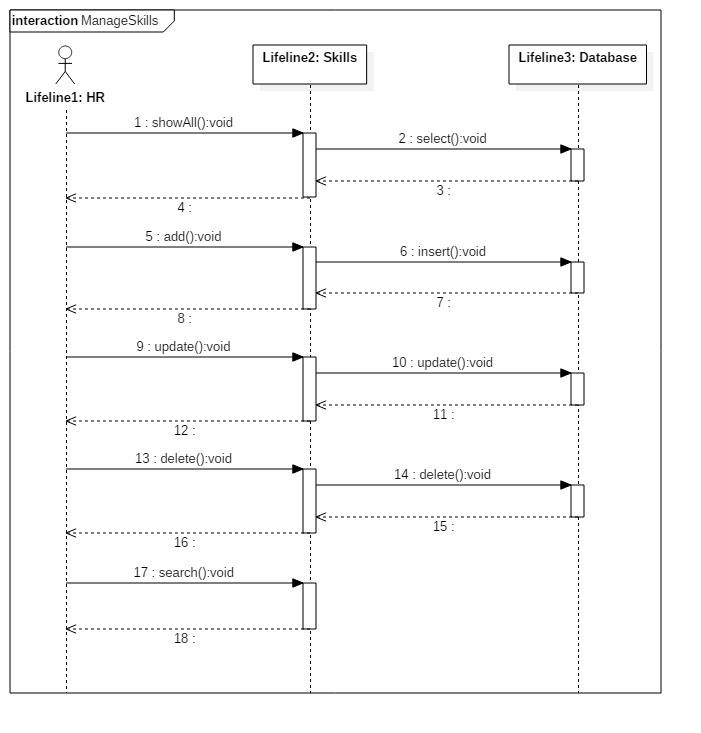
\includegraphics[width=15cm, height=10cm]{Diagram/ManageSkill} \\
\subsection{ER Diagram}
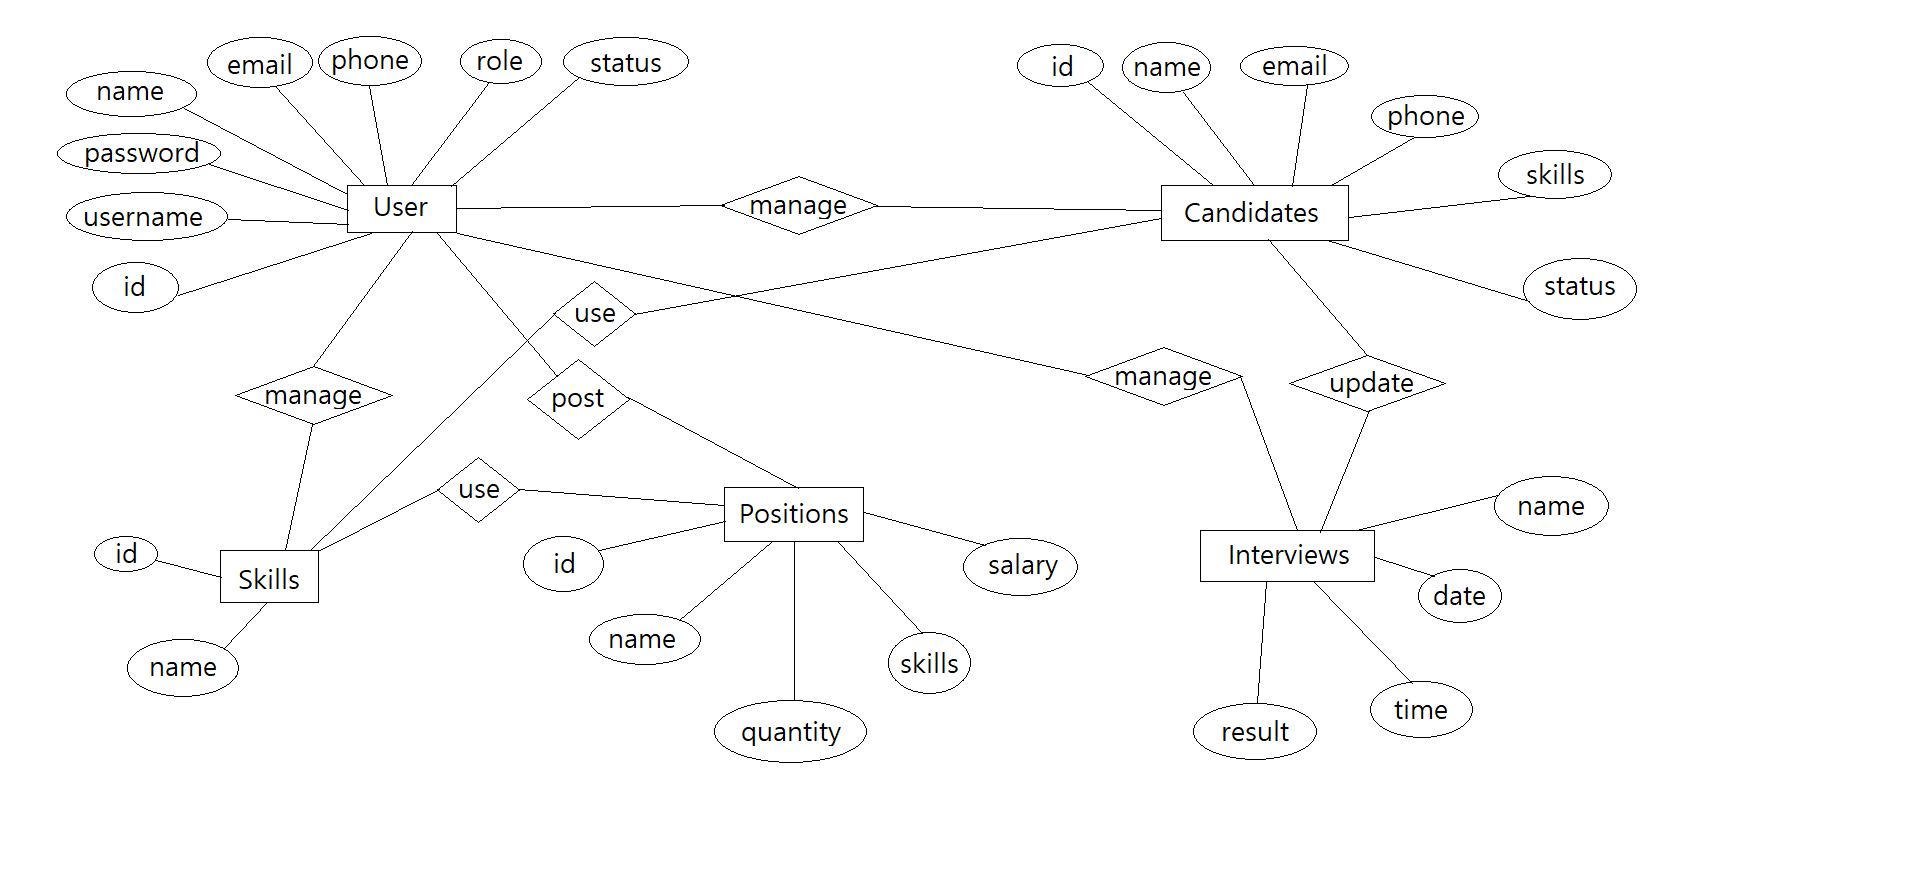
\includegraphics[width=15cm, height=10cm]{Diagram/ERD} \\
\end{document}